\documentclass[10pt,twocolumn,a4paper]{article}

% Pacotes
\usepackage[utf8]{inputenc}
\usepackage[T1]{fontenc}
\usepackage[brazil]{babel}
\usepackage{geometry}
\usepackage{graphicx}
\usepackage{amsmath, amssymb}
\usepackage{booktabs}
\usepackage{cite}
\usepackage{hyperref}
\usepackage{float}
\usepackage{array}
\usepackage{longtable}
\usepackage{xcolor}
\usepackage{listings}
\usepackage{enumitem}
\usepackage{caption}

% Margens
\geometry{left=2cm, right=2cm, top=2cm, bottom=2cm}
\setlength{\columnsep}{0.7cm}

% Configuração de código
\lstset{
    basicstyle=\ttfamily\footnotesize,
    breaklines=true,
    frame=single,
    columns=fullflexible,
    keepspaces=true
}

% Título
\title{\textbf{Análise de Programação Paralela aplicada à busca de substrings em arquivos texto de grande porte}\\
\large Sistemas Distribuídos / Programação Paralela -- UTFPR}

\author{
    Samuel Minuzzo Pereira \\
    \texttt{samuelpereira@utfpr.edu.br}
    \and
    Edilson Daniel de Souza \\
    \texttt{edilsonsouza@alunos.utfpr.edu.br}
}

\date{\today}

\begin{document}

\maketitle

\begin{abstract}
Este trabalho apresenta a implementação e a análise de versões sequenciais e paralelas para o problema de busca de substrings em arquivos texto de grandes. Foram desenvolvidas soluções em C e Java, contemplando uma versão sequencial e uma versão paralela em cada linguagem. Em C, a paralelização foi realizada com OpenMP, enquanto em Java foi utilizada uma abordagem com múltiplas threads por meio de \textit{ExecutorService} (Confirmar depois). O núcleo algorítmico das soluções desenvolvidas pelos autores do trabalho foi baseado no algoritmo Boyer-Moore-Horspool (BMH), adaptado para processamento em blocos e para contagem de ocorrências sobrepostas. Além disso, são discutidas as implementações desenvolvidas pela dupla e as implementações de referência fornecidas pelo colega de trabalho, permitindo uma comparação entre estratégias de mapeamento de arquivo, leitura em blocos, divisão de tarefas e sincronização. Os resultados experimentais são comparados em termos de tempo de execução e \textit{speedup}, buscando avaliar a eficiência das abordagens adotadas em diferentes tamanhos de entrada e diferentes níveis de paralelismo.
\end{abstract}

\textbf{Palavras-chave:} Programação Paralela, Boyer-Moore-Horspool, OpenMP, Threads, Busca de Substrings, Desempenho.

% ------------------------------------------------

\section{Introdução}

A busca por padrões em texto é um problema clássico da computação, presente em aplicações como indexação de documentos, sistemas de busca, mineração de dados, bioinformática, análise forense, processamento de grandes logs e monitoramento de sistemas. À medida que o volume de dados cresce, abordagens simples de comparação caractere a caractere tornam-se progressivamente mais custosas, tornando necessário o uso de algoritmos mais eficientes e de técnicas de paralelização.

Neste trabalho, foi estudado o problema de localizar e contar ocorrências de substrings em arquivos texto de grande porte, com tamanhos variando de frações de gigabyte até múltiplos gigabytes. O foco da análise foi avaliar como diferentes escolhas de implementação impactam o desempenho computacional, especialmente quando o problema é executado de forma sequencial e paralela.

A motivação do trabalho está diretamente associada à necessidade de compreender, na prática, como conceitos de programação paralela podem ser aplicados a um problema real de processamento intensivo de dados. Além disso, o tema permite comparar dois aspectos importantes da computação de alto desempenho: a eficiência algorítmica e a eficiência da exploração de paralelismo.

O objetivo geral do trabalho é implementar, executar e comparar quatro versões do problema:

\begin{itemize}[leftmargin=*]
    \item versão sequencial em Java;
    \item versão paralela em Java com threads;
    \item versão sequencial em C;
    \item versão paralela em C com OpenMP.
\end{itemize}

Adicionalmente, o trabalho também considera a solução do colega como referência comparativa, permitindo discutir diferentes estratégias de implementação para o mesmo problema. Dessa forma, além da comparação entre linguagens e entre versões sequenciais e paralelas, também é possível analisar diferenças de projeto entre soluções distintas para o mesmo objetivo computacional.

% ------------------------------------------------

\section{Descrição do Problema}

O problema tratado neste trabalho consiste em contar o número de ocorrências de uma determinada substring em um arquivo texto de grande porte. Diferentemente de uma busca por ``palavra inteira'', a proposta adotada considera ocorrências de substring no sentido literal, isto é, toda sequência de bytes compatível com o padrão buscado deve ser contabilizada, inclusive ocorrências sobrepostas.

\subsection{Definição formal}

Dado:

\begin{itemize}[leftmargin=*]
    \item um arquivo texto $T$ com comprimento $n$ bytes;
    \item uma substring padrão $P$ com comprimento $m$ bytes, com $1 \leq m \leq n$;
\end{itemize}

deve-se determinar o número de índices $i$ tais que:

\[
T[i..i+m-1] = P
\]

onde $0 \leq i \leq n-m$.

No contexto deste trabalho, a entrada é tratada como uma sequência de bytes. Essa decisão simplifica a implementação e torna a solução compatível com diferentes tamanhos de arquivo, embora implique que a interpretação semântica de caracteres multibyte em UTF-8 não seja o foco principal da contagem.

\subsection{Entrada}

A entrada do problema é composta por:

\begin{itemize}[leftmargin=*]
    \item o caminho para um arquivo texto;
    \item a substring que será procurada;
    \item no caso das versões paralelas, o número de threads a serem utilizadas.
\end{itemize}

\subsection{Saída}

A saída consiste em:

\begin{itemize}[leftmargin=*]
    \item o número total de ocorrências encontradas;
    \item o tempo de execução da versão sequencial;
    \item o tempo de execução da versão paralela;
    \item o \textit{speedup} calculado a partir desses tempos.
\end{itemize}

\subsection{Complexidade esperada}

Uma solução ingênua para o problema, baseada em comparação direta do padrão em todas as posições possíveis, possui complexidade de pior caso aproximadamente $O(n \cdot m)$. Para arquivos muito grandes, esse custo pode tornar-se significativo.

Neste trabalho, a principal estratégia algorítmica adotada nas implementações dos autores foi o algoritmo Boyer-Moore-Horspool, que, embora também possa apresentar pior caso $O(n \cdot m)$, tende a apresentar desempenho muito melhor na prática para textos reais, pois utiliza deslocamentos que permitem pular posições do texto sem comparação completa em todas elas.

Além da eficiência algorítmica, o problema também se mostrou adequado para paralelização, desde que o espaço de busca seja dividido cuidadosamente e que as fronteiras entre blocos sejam tratadas de forma correta para evitar perda ou dupla contagem de ocorrências.

% ------------------------------------------------

\section{Fundamentação Teórica}

\subsection{Busca de padrões em texto}

A busca de padrões em texto pode ser realizada por diferentes estratégias. A abordagem mais simples consiste em alinhar o padrão em cada posição do texto e comparar os caracteres sequencialmente. Essa solução é conceitualmente simples, porém pouco eficiente para arquivos muito grandes, especialmente quando o padrão possui mais de um caractere.

Algoritmos mais avançados exploram pré-processamento do padrão para reduzir o número de comparações efetivas. Entre os algoritmos clássicos, destacam-se Boyer-Moore, Knuth-Morris-Pratt e Boyer-Moore-Horspool. Neste trabalho, o algoritmo central das implementações autorais foi o Boyer-Moore-Horspool, por apresentar boa relação entre simplicidade de implementação e desempenho prático.

\subsection{O algoritmo Boyer-Moore-Horspool (BMH)}

O algoritmo Boyer-Moore-Horspool é uma variação simplificada do algoritmo de Boyer-Moore. Sua principal ideia é comparar o padrão com o texto a partir do último caractere do padrão. Quando ocorre uma discrepância, em vez de avançar apenas uma posição, o algoritmo usa uma tabela de deslocamentos para determinar quantas posições o padrão pode ser movido com segurança.

\subsubsection{Pré-processamento}

Seja $P$ o padrão de comprimento $m$. Constrói-se uma tabela de deslocamento para todos os possíveis valores de byte. Inicialmente, todos os deslocamentos recebem o valor $m$. Em seguida, para cada posição do padrão, exceto a última, define-se:

\[
shift[P[i]] = m - 1 - i
\]

para $0 \leq i < m-1$.

Essa tabela informa o quanto o padrão pode ser deslocado quando o caractere alinhado ao final da janela de comparação causa um erro de correspondência.

\subsubsection{Funcionamento}

Em cada etapa:

\begin{enumerate}[leftmargin=*]
    \item alinha-se o padrão a uma posição do texto;
    \item compara-se o último caractere do padrão com o caractere correspondente do texto;
    \item se houver coincidência, prossegue-se a comparação de trás para frente;
    \item se houver erro, consulta-se a tabela de deslocamento e o padrão é movido adequadamente.
\end{enumerate}

\subsubsection{Exemplo conceitual}

Suponha o padrão \texttt{como}. O último caractere é \texttt{o}. Ao alinhar o padrão a uma posição do texto, o algoritmo observa primeiramente o byte correspondente a \texttt{o}. Se esse byte não coincidir, não é necessário comparar os demais bytes; o deslocamento é determinado diretamente pela tabela.

Esse comportamento reduz significativamente o número de comparações, principalmente quando o alfabeto do texto é relativamente amplo e o padrão não aparece com extrema frequência.

\subsubsection{Vantagens do BMH}

As principais vantagens do BMH são:

\begin{itemize}[leftmargin=*]
    \item implementação relativamente simples;
    \item bom desempenho prático em busca de substrings;
    \item redução do número de comparações em relação à busca direta;
    \item excelente adaptação para tratamento byte a byte;
    \item boa integração com leitura em blocos para arquivos grandes.
\end{itemize}

\subsubsection{Desvantagens do BMH}

Como limitações, destacam-se:

\begin{itemize}[leftmargin=*]
    \item pior caso ainda proporcional a $O(n \cdot m)$;
    \item necessidade de cuidado extra ao dividir o texto para processamento paralelo;
    \item menor aproveitamento dos saltos quando o padrão é muito curto, especialmente de tamanho 1 (pior cenário).
\end{itemize}

% melhorar essa parte dando exemplos mais claros de como foi realizada a paralelização
\subsection{Paralelização do problema}

A paralelização da busca de substrings não é trivial, pois o texto não pode ser simplesmente dividido em partes independentes sem considerar as fronteiras. Se uma ocorrência começar no final de um bloco e terminar no início do próximo, ela poderá ser perdida.

Para resolver esse problema, as implementações paralelas adotaram estratégias de sobreposição ou de propriedade de intervalo:

\begin{itemize}[leftmargin=*]
    \item \textbf{sobreposição entre blocos:} cada bloco é lido com alguns bytes adicionais do bloco seguinte;
    \item \textbf{intervalo de propriedade:} cada thread pode inspecionar além do seu limite, mas só contabiliza ocorrências cujo índice inicial pertence ao seu intervalo.
\end{itemize}

Esse cuidado é essencial para garantir correção na contagem.

% ------------------------------------------------

\section{Implementações}

Esta seção descreve as quatro versões consideradas no trabalho, bem como as decisões de projeto adotadas. Também são discutidas as soluções de referência do colega, utilizadas como base comparativa.

\subsection{Visão geral das implementações}

As implementações foram organizadas em duas linguagens, C e Java, e em dois modos de execução, sequencial e paralelo. Em ambos os casos, o problema atacado foi o mesmo: contagem de ocorrências de substring em arquivos de grande porte.

As soluções desenvolvidas pelos autores adotaram uma base algorítmica comum:
\begin{itemize}[leftmargin=*]
    \item busca por substring literal;
    \item tratamento de ocorrências sobrepostas;
    \item leitura em blocos (\textit{chunks});
    \item preservação de uma região de sobreposição entre blocos;
    \item uso de Boyer-Moore-Horspool como núcleo de busca.
\end{itemize}

Já as soluções do colega adotaram uma estratégia distinta em alguns casos, especialmente em C, empregando mapeamento de arquivo em memória e uso de OpenMP diretamente sobre regiões do arquivo.

\subsection{Versão Sequencial em Java}

A versão sequencial em Java desenvolvida pelos autores foi construída com foco em manter a mesma lógica algorítmica da versão em C, permitindo uma comparação justa entre linguagens.

\subsubsection{Estrutura da solução}

A implementação realiza:

\begin{enumerate}[leftmargin=*]
    \item leitura do arquivo em blocos com \texttt{BufferedInputStream};
    \item conversão da substring em vetor de bytes;
    \item construção da tabela de deslocamentos do BMH;
    \item execução da busca em cada bloco;
    \item preservação dos últimos $m-1$ bytes entre blocos.
\end{enumerate}

Essa abordagem evita a necessidade de carregar o arquivo inteiro em memória, o que é importante para entradas de múltiplos gigabytes.

\subsubsection{Motivação da escolha}

A escolha de leitura em blocos em Java foi motivada por:

\begin{itemize}[leftmargin=*]
    \item portabilidade da implementação;
    \item controle explícito da memória utilizada;
    \item possibilidade de manter a mesma semântica do código em C;
    \item facilidade de adaptação futura para a versão paralela.
\end{itemize}

\subsubsection{Vantagens}

\begin{itemize}[leftmargin=*]
    \item boa organização estrutural;
    \item menor risco de esgotamento de memória;
    \item boa correspondência conceitual com a versão sequencial em C;
    \item fácil integração com o sistema de automação dos testes.
\end{itemize}

\subsubsection{Desvantagens}

\begin{itemize}[leftmargin=*]
    \item maior overhead da máquina virtual Java;
    \item custo adicional de gerenciamento de memória;
    \item desempenho inferior ao C em operações intensivas de baixo nível.
\end{itemize}

\subsection{Versão Sequencial em C}

A versão sequencial em C foi construída com a mesma ideia central da implementação em Java, porém explorando recursos de mais baixo nível da linguagem, como controle manual de memória, alinhamento de buffer e maior proximidade do hardware.

\subsubsection{Estrutura da solução}

A solução sequencial em C:

\begin{enumerate}[leftmargin=*]
    \item abre o arquivo em modo binário;
    \item ajusta um buffer de E/S com \texttt{setvbuf};
    \item monta a tabela de deslocamentos do BMH;
    \item lê o arquivo em blocos grandes;
    \item preserva uma região de sobreposição entre blocos;
    \item executa a busca sequencial no bloco.
\end{enumerate}

Além disso, a implementação faz uso de um tratamento específico para padrões de tamanho 1, contando ocorrências de um único byte de forma direta, o que é vantajoso para palavras muito curtas.

\subsubsection{Particularidades}

A versão em C permite maior controle sobre:
\begin{itemize}[leftmargin=*]
    \item tamanho dos buffers;
    \item estratégia de alinhamento em memória;
    \item custo de abstrações;
    \item medição mais precisa do tempo de execução.
\end{itemize}

\subsubsection{Vantagens}

\begin{itemize}[leftmargin=*]
    \item maior eficiência de baixo nível;
    \item menor overhead de execução;
    \item melhor aproveitamento de memória e cache;
    \item base sólida para paralelização com OpenMP.
\end{itemize}

\subsubsection{Desvantagens}

\begin{itemize}[leftmargin=*]
    \item maior complexidade de implementação;
    \item maior responsabilidade do programador com memória e corretude;
    \item menor portabilidade imediata em comparação com Java quando há dependências específicas de compilação.
\end{itemize}

\subsection{Versão Paralela com Threads (Java)}

A versão paralela em Java foi desenvolvida preservando a lógica geral de leitura em blocos e BMH, mas introduzindo paralelização na etapa de processamento do bloco.

\subsubsection{Estratégia de paralelização}

A ideia central foi dividir o espaço de possíveis posições iniciais válidas do padrão dentro do bloco entre diferentes threads. Cada thread recebe um intervalo de propriedade. Ela pode inspecionar bytes além do seu limite final, mas só contabiliza uma ocorrência se o índice inicial da ocorrência pertencer ao intervalo que lhe foi atribuído.

Esse método é importante porque evita:

\begin{itemize}[leftmargin=*]
    \item perda de ocorrências na fronteira entre threads;
    \item dupla contagem da mesma ocorrência.
\end{itemize}

\subsubsection{Divisão de tarefas}

A divisão foi feita de forma aproximadamente uniforme entre as threads, com base no número total de posições iniciais válidas para o padrão. Para coordenar a execução, foi utilizado \texttt{ExecutorService}, responsável por criar e gerenciar um conjunto fixo de threads.

\subsubsection{Sincronização}

A sincronização explícita foi minimizada, pois cada tarefa retorna uma contagem local, e a soma final é realizada após a obtenção dos resultados das \textit{futures}. Isso reduz a necessidade de regiões críticas frequentes e tende a melhorar o desempenho.

\subsubsection{Vantagens}

\begin{itemize}[leftmargin=*]
    \item paralelização relativamente limpa e bem encapsulada;
    \item boa correspondência conceitual com a versão OpenMP em C;
    \item facilidade de ajuste do número de threads;
    \item menor risco de condições de corrida no contador global.
\end{itemize}

\subsubsection{Desvantagens}

\begin{itemize}[leftmargin=*]
    \item maior overhead de criação e gerenciamento de tarefas;
    \item dependência do comportamento do coletor de lixo e da JVM;
    \item possível custo adicional de sincronização interna do \texttt{ExecutorService}.
\end{itemize}

\subsection{Versão Paralela com OpenMP (C)}

A versão paralela em C utilizou OpenMP para paralelizar a busca em cada bloco do arquivo. O princípio de divisão do espaço de busca foi semelhante ao adotado na versão Java, mas com a vantagem de um ambiente de execução mais leve e de menor overhead.

\subsubsection{Uso de \texttt{\#pragma omp}}

A paralelização foi implementada com diretivas \texttt{\#pragma omp parallel for reduction(+:total)}, permitindo que diferentes threads processem subintervalos do espaço de busca em paralelo e que as contagens parciais sejam acumuladas de forma segura por meio de \textit{reduction}.

\subsubsection{Tipo de paralelismo}

O paralelismo utilizado é do tipo \textit{data parallelism}, no qual diferentes threads executam a mesma operação sobre diferentes partes do conjunto de dados.

\subsubsection{Tratamento das fronteiras}

A mesma ideia de intervalo de propriedade foi aplicada: cada thread recebe um conjunto de posições iniciais válidas e pode inspecionar além da sua região, mas apenas contabiliza as ocorrências que efetivamente se iniciam dentro do seu intervalo.

\subsubsection{Vantagens}

\begin{itemize}[leftmargin=*]
    \item baixo overhead em relação a outras abordagens de paralelização;
    \item sintaxe direta e integrada ao C;
    \item excelente controle do número de threads;
    \item desempenho geralmente superior ao Java em tarefas intensivas de CPU.
\end{itemize}

\subsubsection{Desvantagens}

\begin{itemize}[leftmargin=*]
    \item exige compilador com suporte a OpenMP;
    \item maior sensibilidade à arquitetura e ao ambiente de execução;
    \item necessidade de cuidado com equilíbrio de carga e efeitos de memória compartilhada.
\end{itemize}

\subsection{Implementações de referência do colega}

Além das implementações desenvolvidas pelos autores, também foram analisadas as soluções do colega de trabalho, utilizadas como base comparativa.

\subsubsection{Solução em C do colega}

A solução do colega em C utilizou mapeamento de arquivo em memória (\texttt{mmap} em Unix e \texttt{MapViewOfFile} em Windows) e uma varredura sobre os bytes mapeados. Na versão paralela, o arquivo foi dividido em regiões processadas por diferentes threads via OpenMP, com uma pequena sobreposição para reduzir o risco de perda de ocorrências na fronteira.

Essa abordagem apresenta vantagens importantes:
\begin{itemize}[leftmargin=*]
    \item acesso eficiente ao arquivo por meio do sistema operacional;
    \item ausência de cópias explícitas de grandes blocos para buffers intermediários;
    \item implementação compacta para leitura de arquivos grandes.
\end{itemize}

Por outro lado, a abordagem também requer cuidado:
\begin{itemize}[leftmargin=*]
    \item forte dependência do comportamento do sistema operacional e do subsistema de memória virtual;
    \item risco de gargalos em regiões de fronteira;
    \item necessidade de garantir corretude em divisões paralelas.
\end{itemize}

\subsubsection{Solução em Java do colega}

A implementação do colega em Java foi baseada em \texttt{RandomAccessFile}, \texttt{FileChannel} e \texttt{ByteBuffer.allocateDirect}. A versão sequencial percorre os bytes do arquivo por meio de buffers diretos, enquanto a versão paralela divide o arquivo em partes entre threads e utiliza sincronização controlada para agregar resultados.

Essa abordagem tem como mérito explorar diretamente recursos de E/S mais próximos do sistema operacional, o que pode ser vantajoso em determinadas situações. Em contrapartida, o tratamento correto das fronteiras entre partes e o custo de coordenação entre threads continuam sendo pontos críticos para o desempenho global.

% ------------------------------------------------

\section{Metodologia de Avaliação}

\subsection{Ambiente de Testes}

Todos os experimentos foram executados na máquina do autor, um notebook \textbf{Acer Predator Helios Neo 16 (PHN16-71)}. Os detalhes completos do ambiente de testes estão descritos abaixo:

\begin{itemize}[leftmargin=*]
    \item Modelo do equipamento: \textbf{Acer Predator Helios Neo 16 (PHN16-71)}
    \item Processador: \textbf{Intel Core i7-13650HX}
    \item Número de núcleos físicos: \textbf{14}
    \item Número de threads lógicas: \textbf{20}
    \item Memória RAM: \textbf{24 GB}
    \item Tipo de armazenamento: \textbf{SSD NVMe Kingston SNV2S1000G (1 TB)}
    \item Sistema operacional: \textbf{Windows 11 Home Single Language 64 bits (10.0.26200)}
    \item Versão do compilador C: \textbf{GCC 15.2.0}
    \item Versão da JVM/JDK: \textbf{OpenJDK 17.0.18 (Temurin)}
\end{itemize}

\subsection{Entradas utilizadas}

Os testes foram conduzidos sobre arquivos texto com diferentes tamanhos, com o objetivo de avaliar escalabilidade e comportamento das soluções em diferentes volumes de dados. Entre os tamanhos considerados, destacam-se:

\begin{itemize}[leftmargin=*]
    \item 0,1 GB
    \item 0,5 GB
    \item 1 GB
    \item 2 GB
    \item 4 GB
    \item 6 GB
    \item 8 GB
    \item 10 GB
    \item 15 GB
\end{itemize}

As palavras de teste foram escolhidas com comprimentos e frequências distintas, incluindo substrings muito curtas e substrings maiores, tais como:

\begin{itemize}[leftmargin=*]
    \item \texttt{a}
    \item \texttt{de}
    \item \texttt{como}
    \item \texttt{itaguai}
    \item \texttt{Bacamarte}
    \item \texttt{Evarista}
\end{itemize}

\subsection{Procedimento experimental}

Para cada combinação de:
\begin{itemize}[leftmargin=*]
    \item arquivo,
    \item palavra,
    \item número de threads,
    \item implementação,
\end{itemize}

foram realizadas múltiplas execuções, e os resultados médios foram armazenados em arquivos CSV para posterior análise e geração de gráficos.

A automação dos testes foi realizada por script em Python, responsável por:
\begin{itemize}[leftmargin=*]
    \item invocar os programas em C e Java;
    \item repetir cada experimento;
    \item coletar tempos sequenciais e paralelos;
    \item calcular médias;
    \item exportar resultados tabulados.
\end{itemize}

\subsection{Métricas}

O desempenho foi avaliado com base principalmente em duas métricas:

\begin{enumerate}[leftmargin=*]
    \item tempo de execução;
    \item \textit{speedup}.
\end{enumerate}

O \textit{speedup} foi calculado por:

\begin{equation}
Speedup = \frac{T_s}{T_p}
\end{equation}

Onde:
\begin{itemize}[leftmargin=*]
    \item $T_s$ = tempo sequencial;
    \item $T_p$ = tempo paralelo.
\end{itemize}

Além disso, a corretude da implementação foi verificada comparando-se, sempre que possível, o número de ocorrências retornado pela versão sequencial com o número obtido pela versão paralela.

% ------------------------------------------------
\section{Resultados}

\subsection{Tempo de Execução}

\begin{table}[H]
\centering
\caption{Tempo médio de execução por tamanho de arquivo}
\begin{tabular}{ccccc}
\toprule
Arquivo (GB) & Java Seq & Java Par & C Seq & C Par \\
\midrule
0.1 & 0.164 & 0.123 & 0.087 & 0.055 \\
1 & 1.382 & 0.785 & 0.734 & 0.416 \\
2 & 2.552 & 1.422 & 1.435 & 0.720 \\
4 & 4.858 & 2.618 & 2.762 & 1.336 \\
8 & 9.583 & 5.659 & 5.458 & 2.717 \\
10 & 11.997 & 6.334 & 6.931 & 3.444 \\
15 & 44.107 & 39.829 & 41.749 & 36.802 \\
\bottomrule
\end{tabular}
\end{table}

\subsection{Speedup}

\begin{table}[H]
\centering
\caption{Speedup médio por tamanho de arquivo}
\begin{tabular}{ccc}
\toprule
Arquivo (GB) & Java & C \\
\midrule
0.1 & 1.343 & 1.622 \\
1 & 1.829 & 1.837 \\
2 & 1.876 & 2.132 \\
4 & 1.953 & 2.176 \\
8 & 1.852 & 2.118 \\
10 & 2.008 & 2.121 \\
15 & 1.111 & 1.140 \\
\bottomrule
\end{tabular}
\end{table}

\subsection{Gráficos}

\begin{figure}[H]
\centering
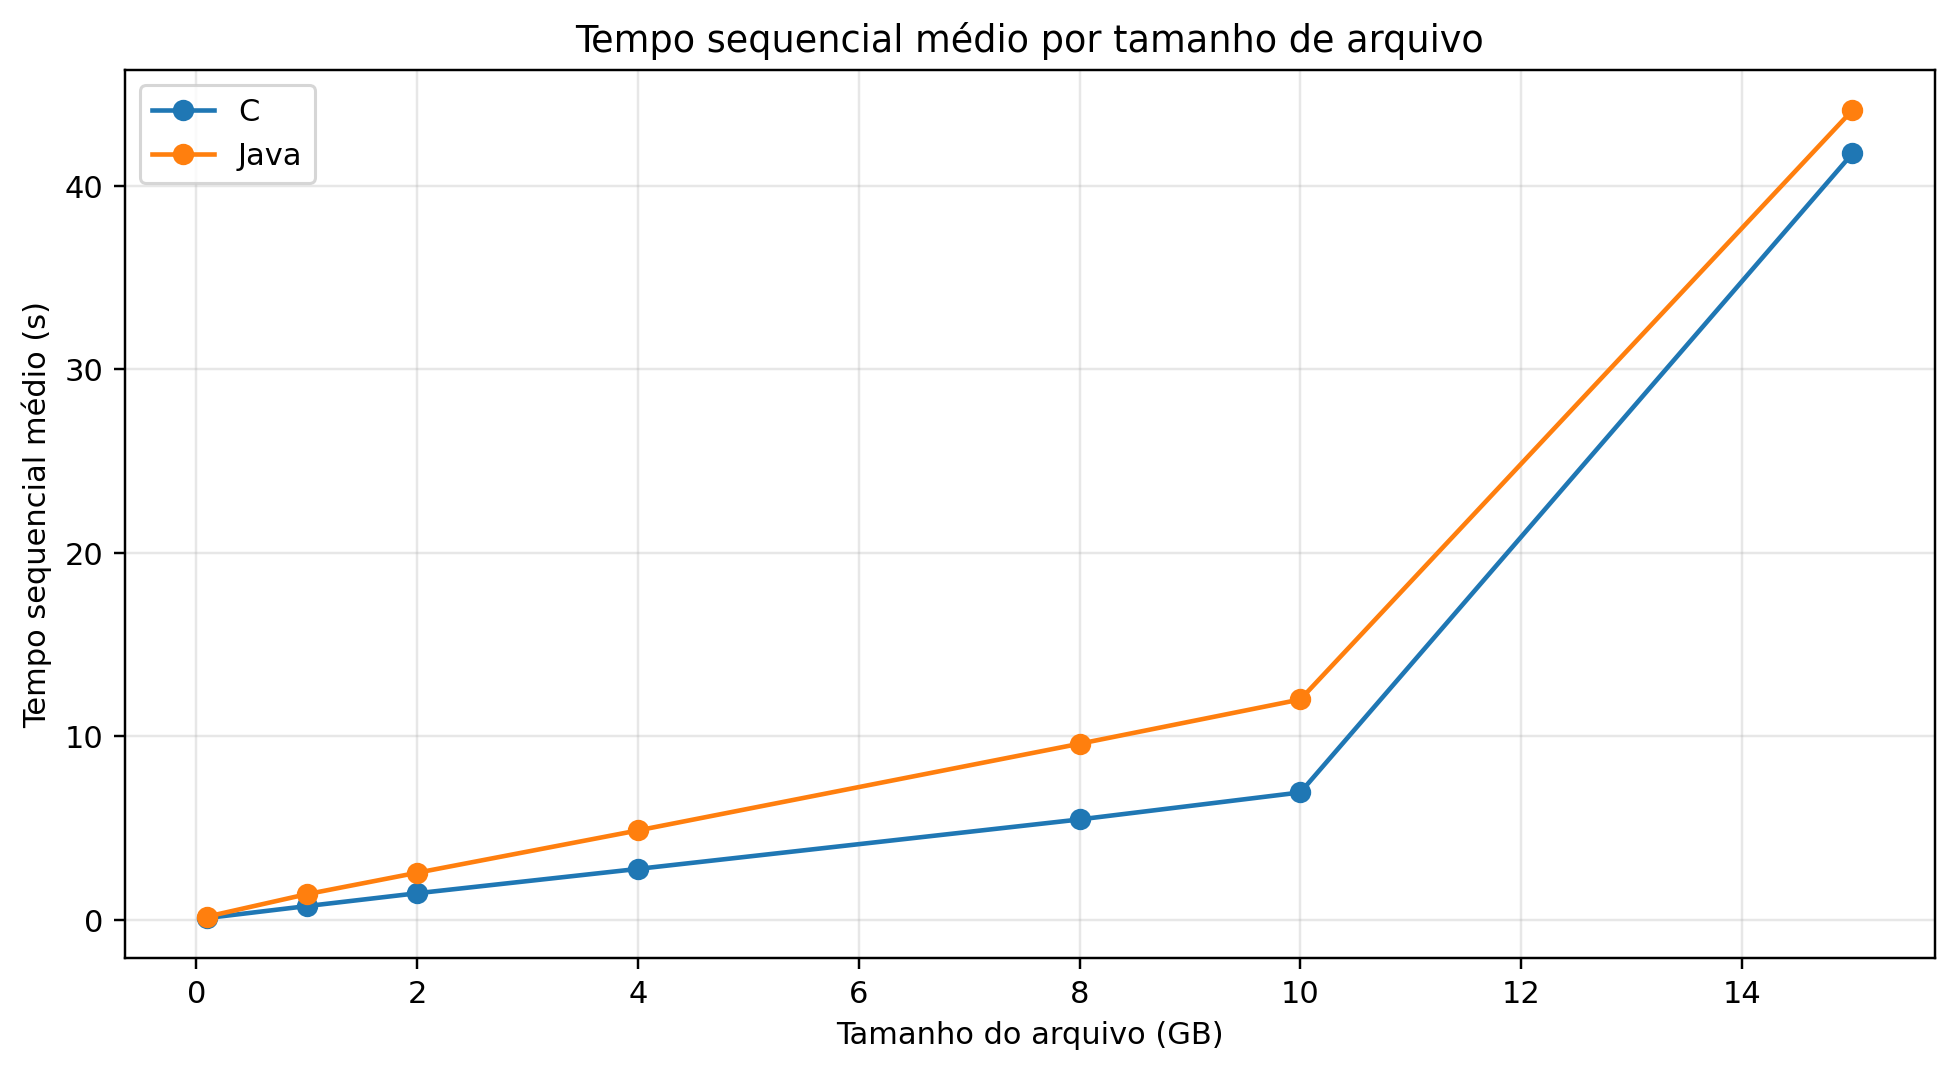
\includegraphics[width=0.45\textwidth]{graficos/tempo_sequencial_por_tamanho.png}
\caption{Tempo sequencial médio por tamanho de arquivo}
\end{figure}

\begin{figure}[H]
\centering
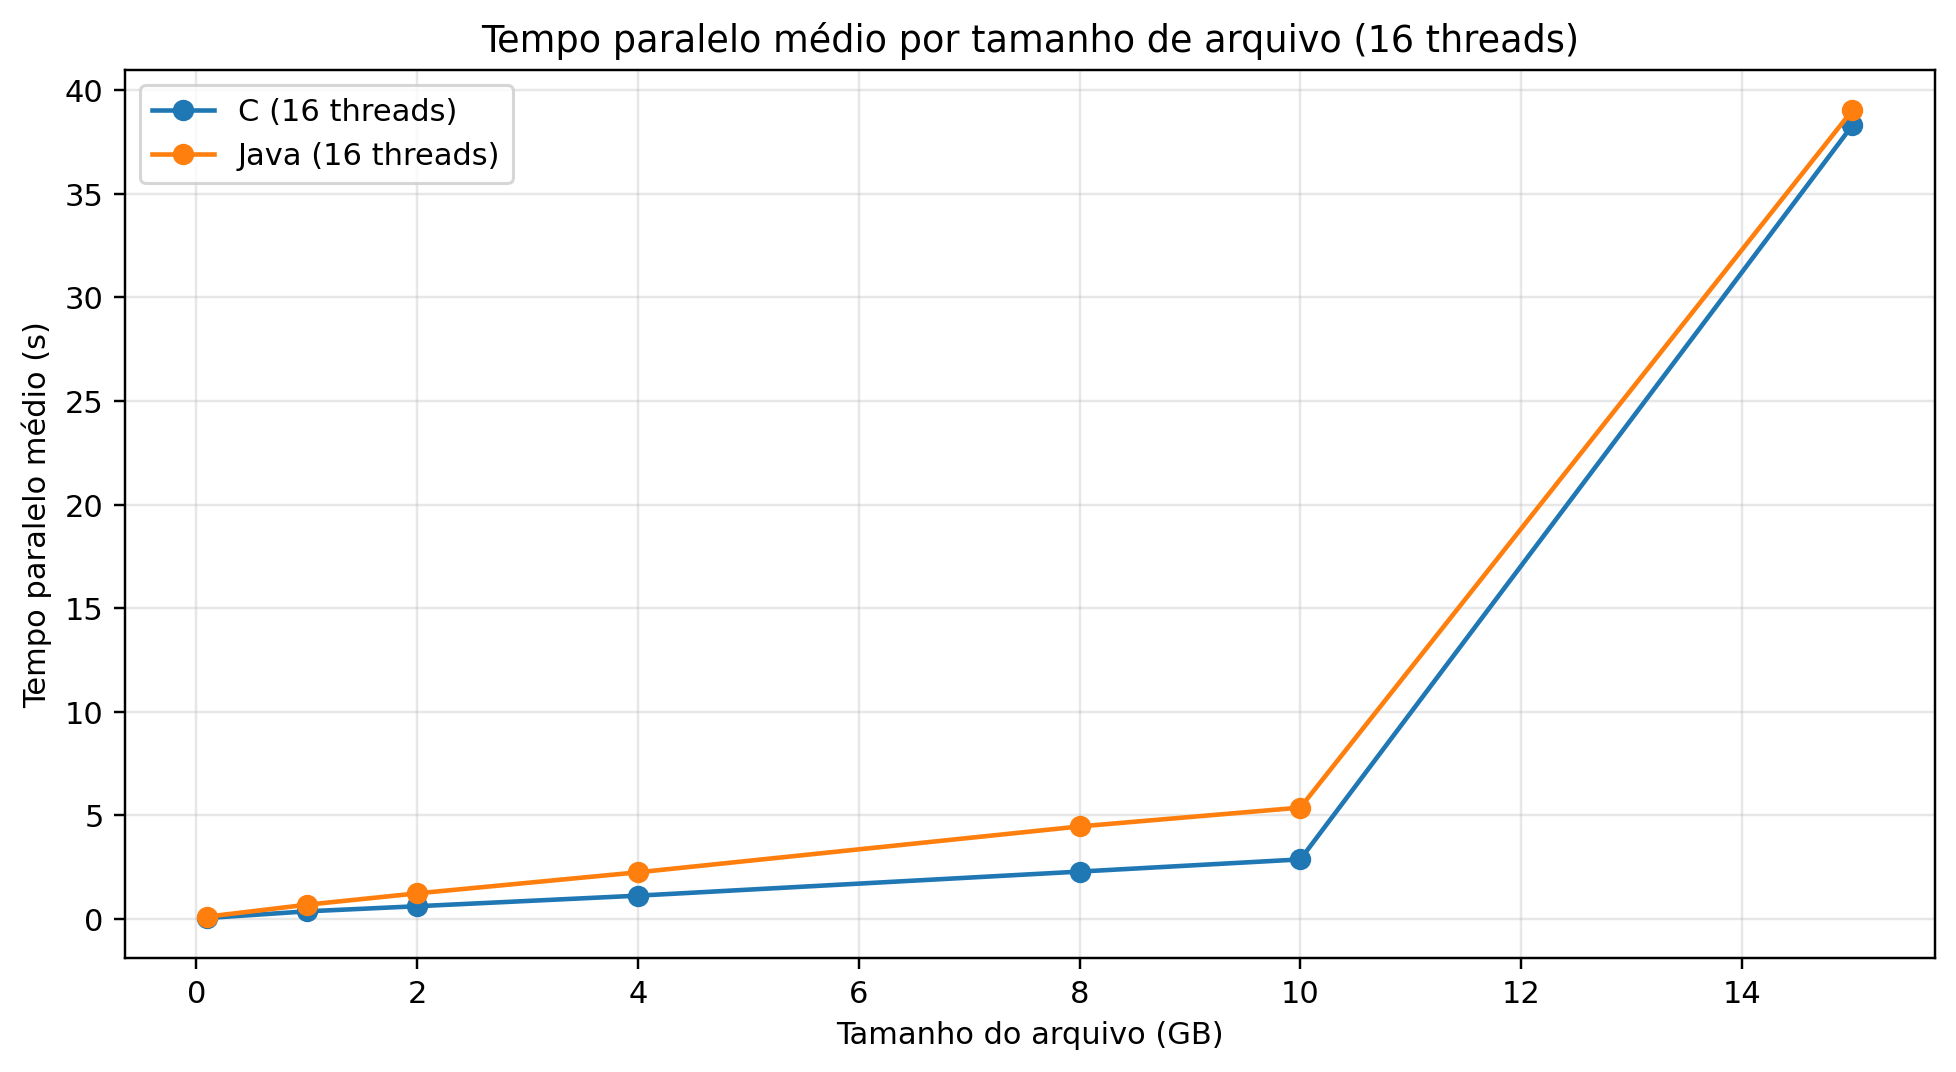
\includegraphics[width=0.45\textwidth]{graficos/tempo_paralelo_por_tamanho_16_threads.png}
\caption{Tempo paralelo médio por tamanho de arquivo (16 threads)}
\end{figure}

\begin{figure}[H]
\centering
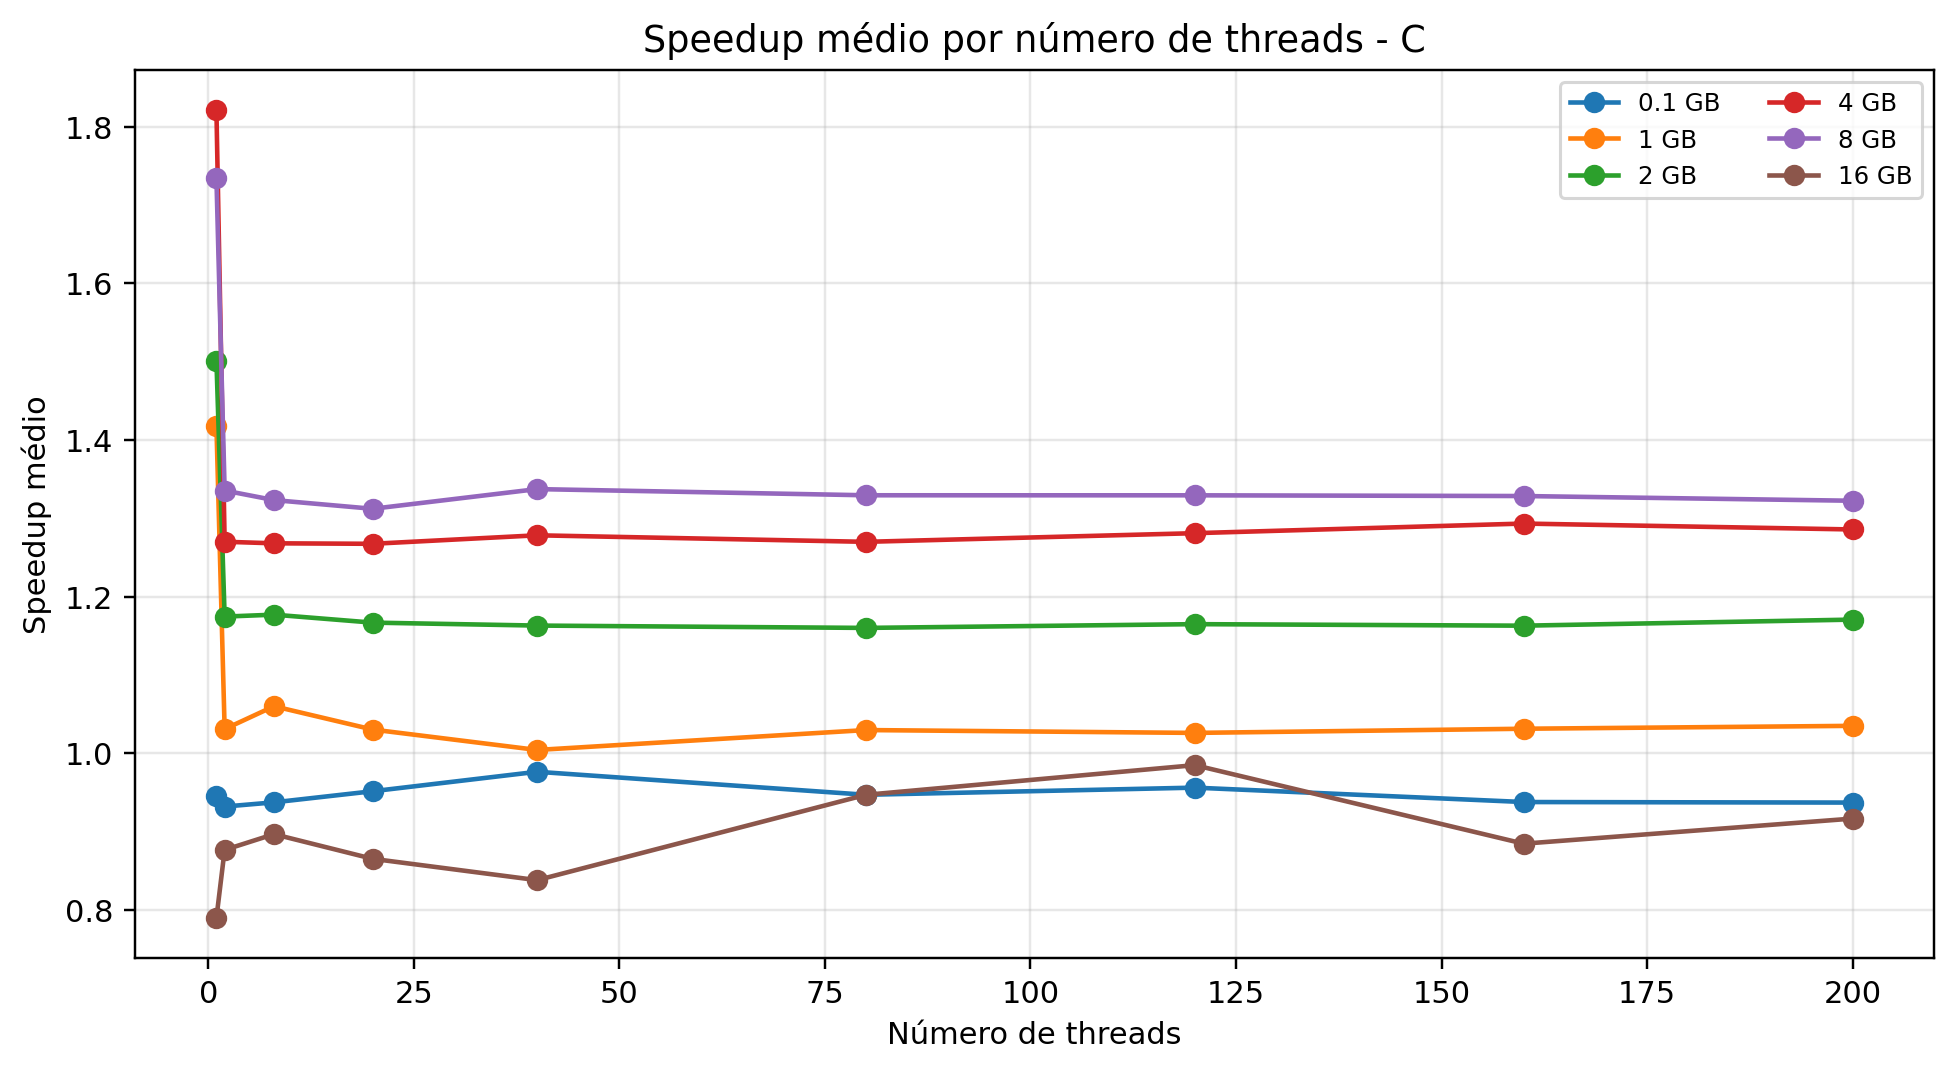
\includegraphics[width=0.45\textwidth]{graficos/speedup_por_threads_C.png}
\caption{Speedup em função do número de threads (C)}
\end{figure}

\begin{figure}[H]
\centering
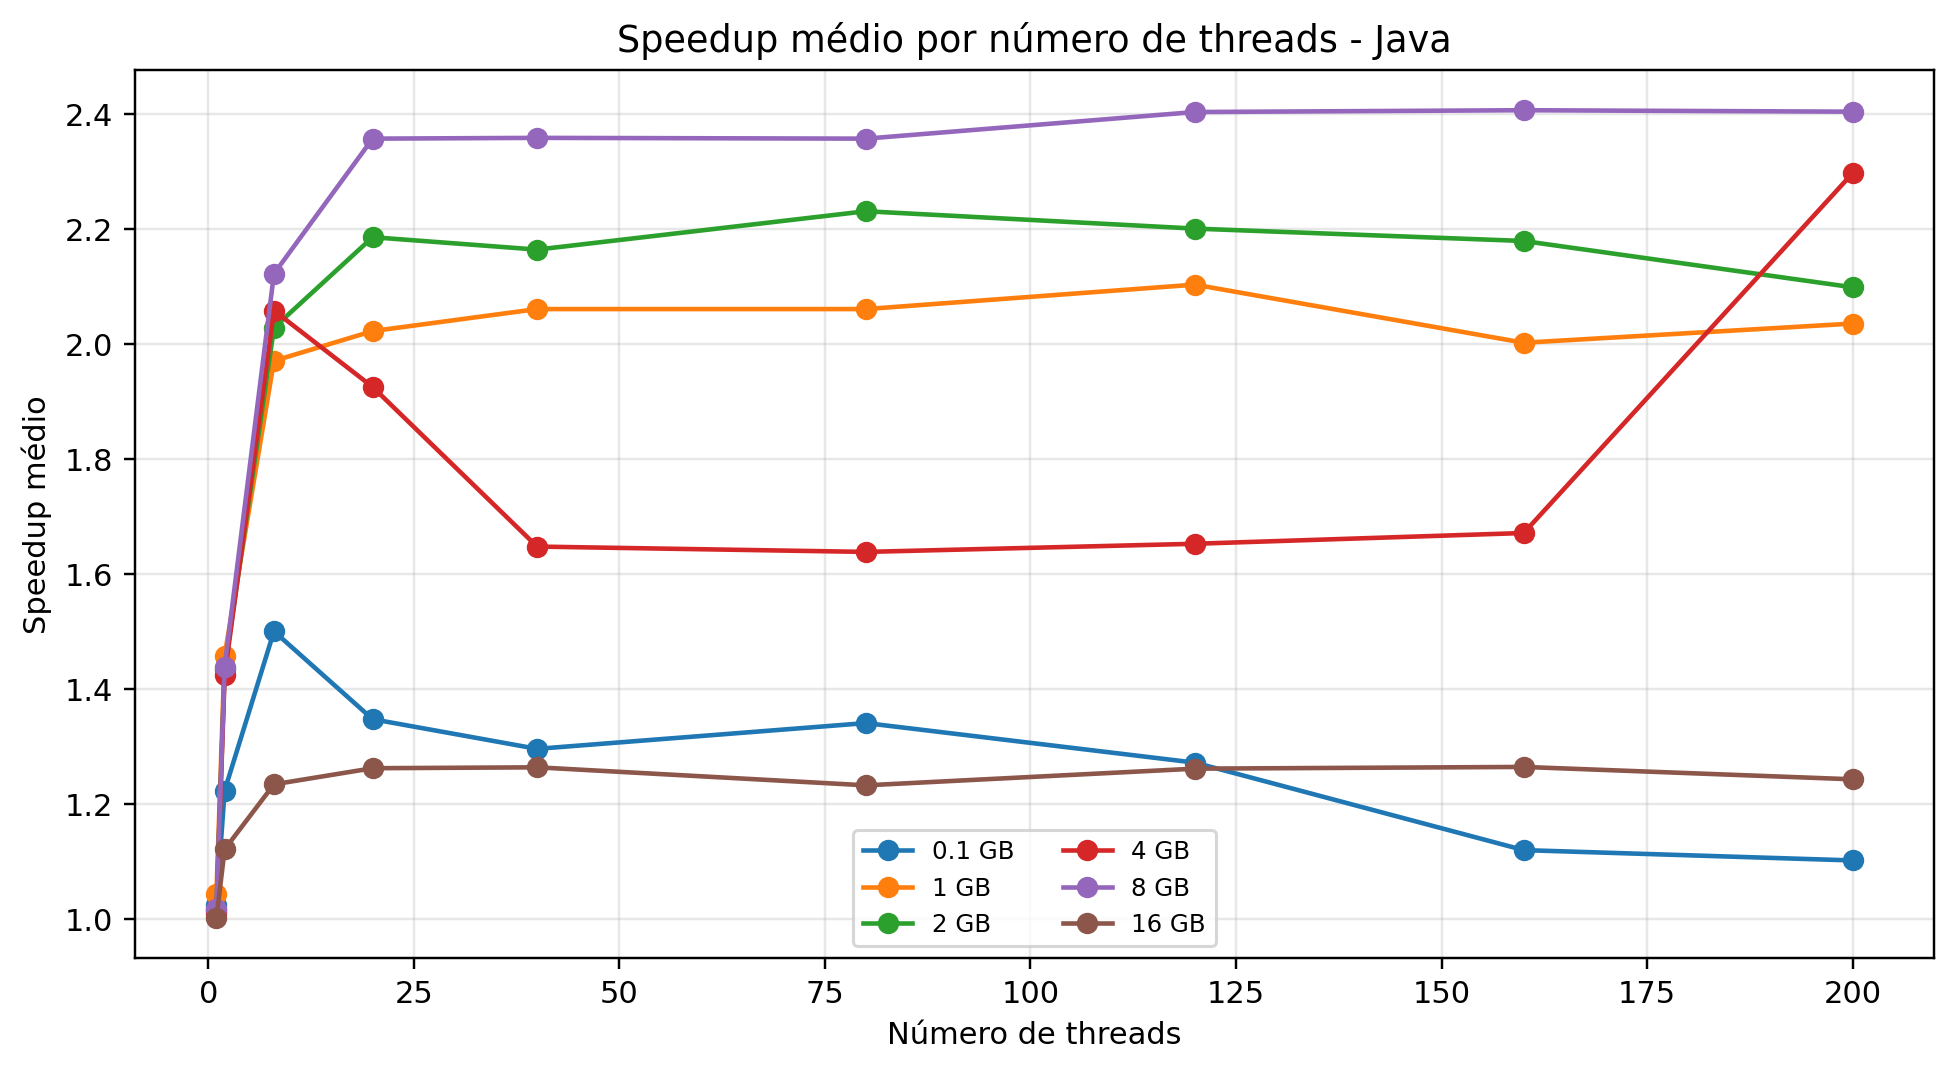
\includegraphics[width=0.45\textwidth]{graficos/speedup_por_threads_Java.png}
\caption{Speedup em função do número de threads (Java)}
\end{figure}

\begin{figure}[H]
\centering
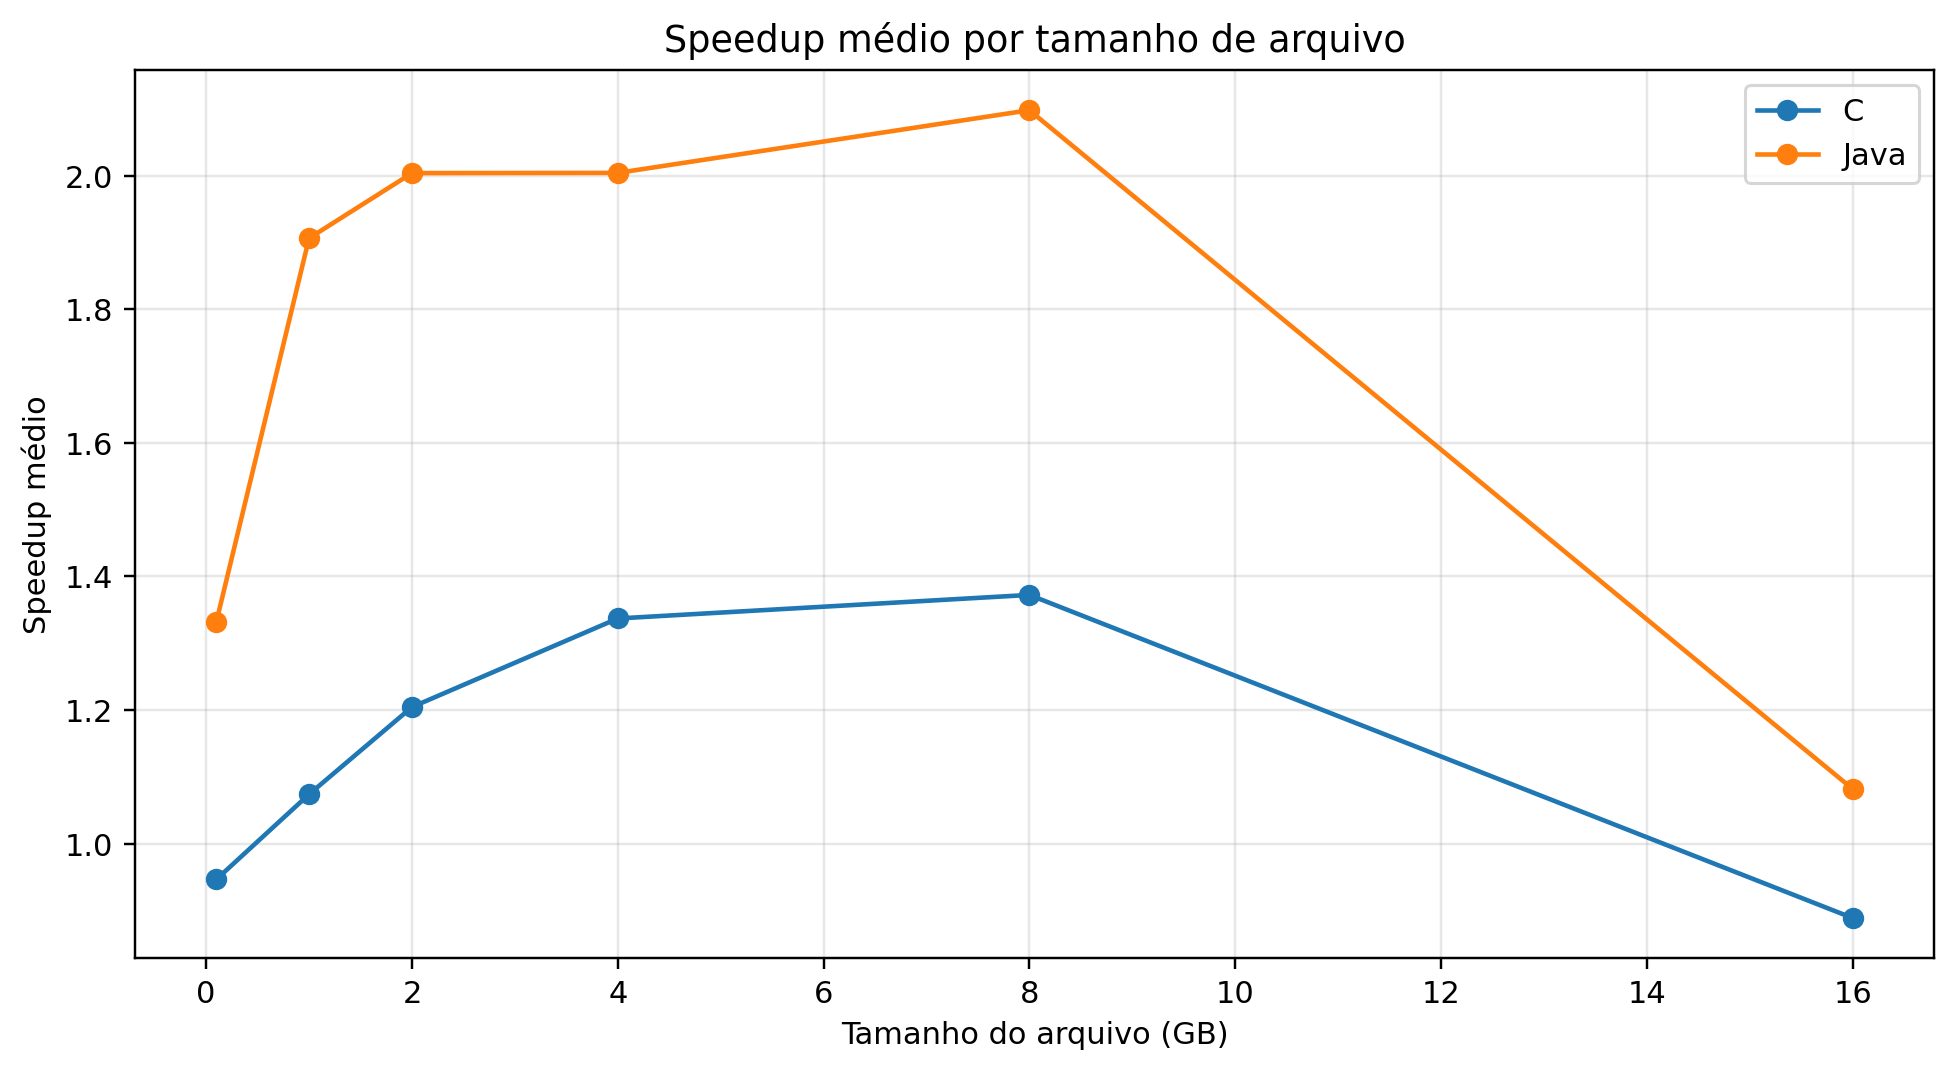
\includegraphics[width=0.45\textwidth]{graficos/speedup_medio_por_tamanho.png}
\caption{Speedup médio por tamanho de arquivo}
\end{figure}

\begin{figure}[H]
\centering
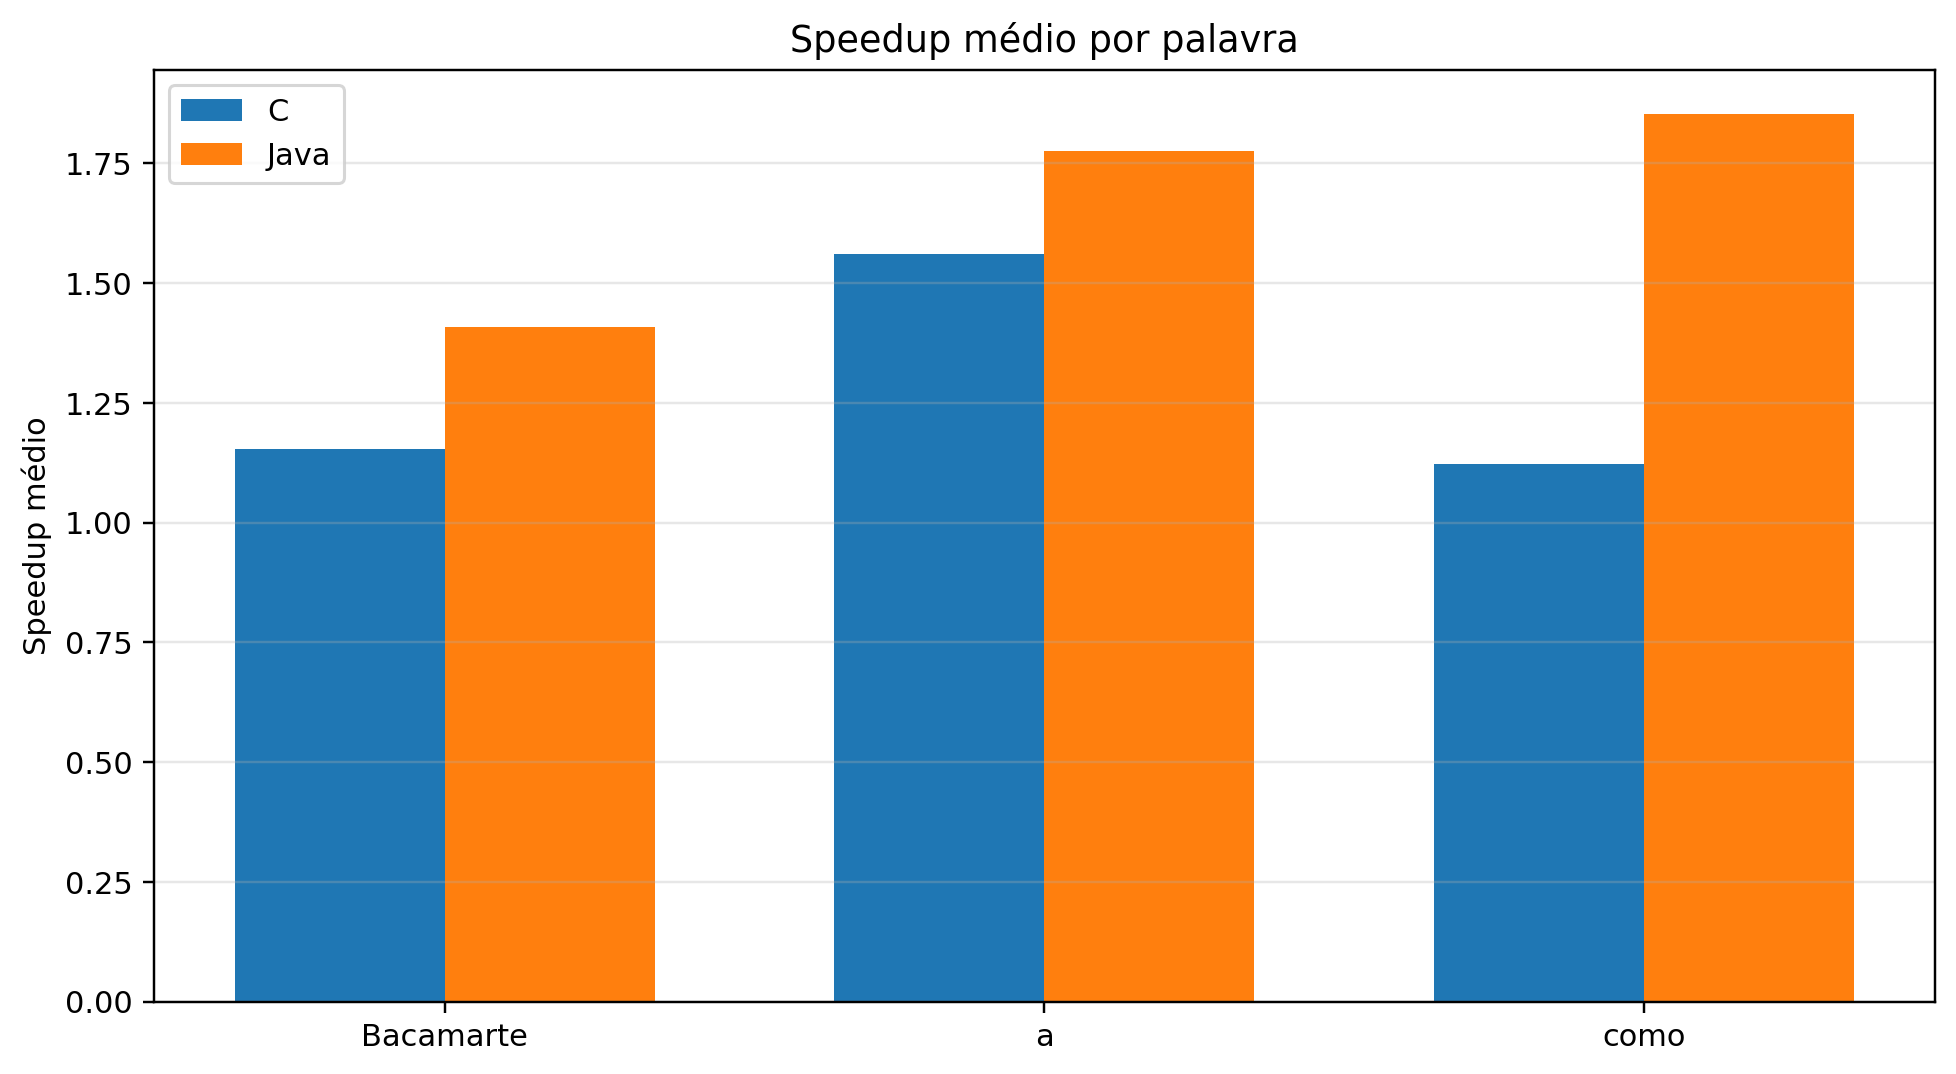
\includegraphics[width=0.45\textwidth]{graficos/speedup_por_palavra.png}
\caption{Speedup médio por palavra}
\end{figure}

\begin{figure}[H]
\centering
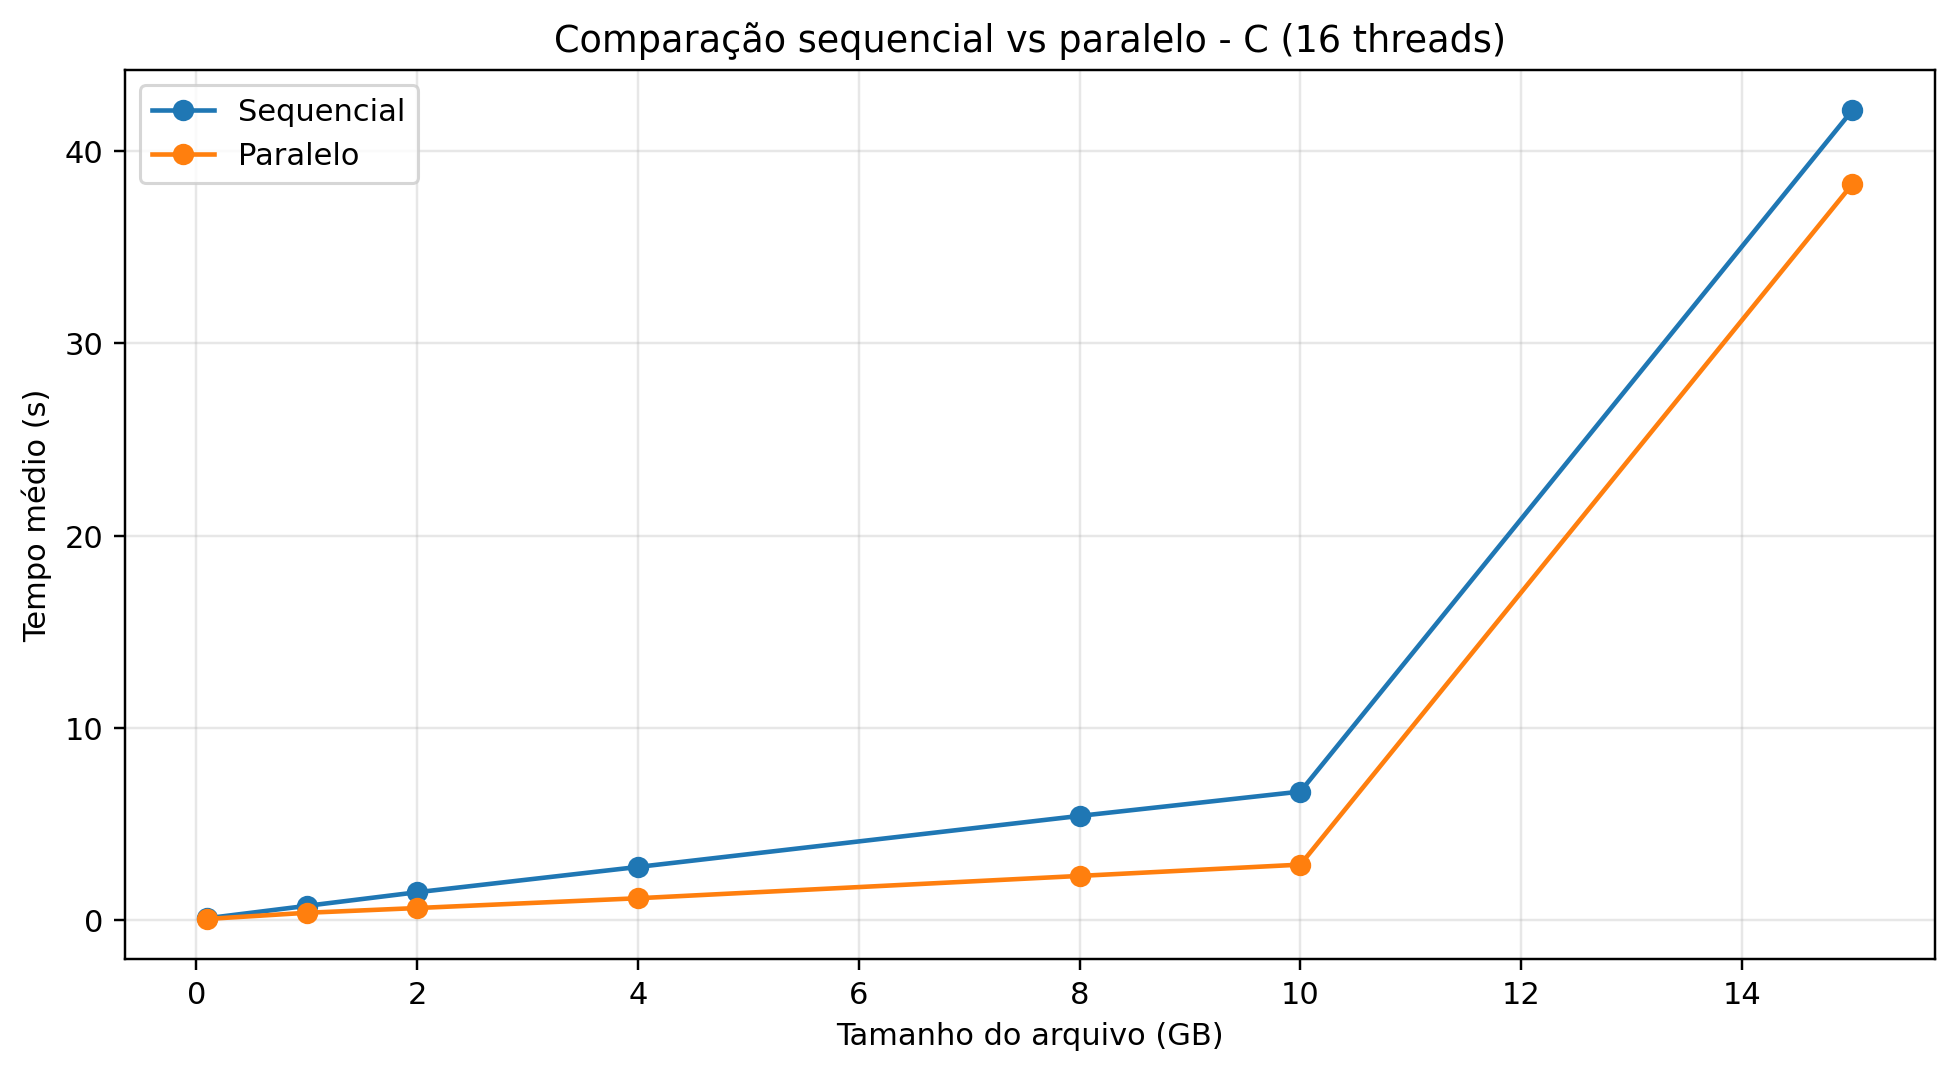
\includegraphics[width=0.45\textwidth]{graficos/comparacao_seq_vs_par_C_16_threads.png}
\caption{Comparação entre execução sequencial e paralela em C}
\end{figure}

\begin{figure}[H]
\centering
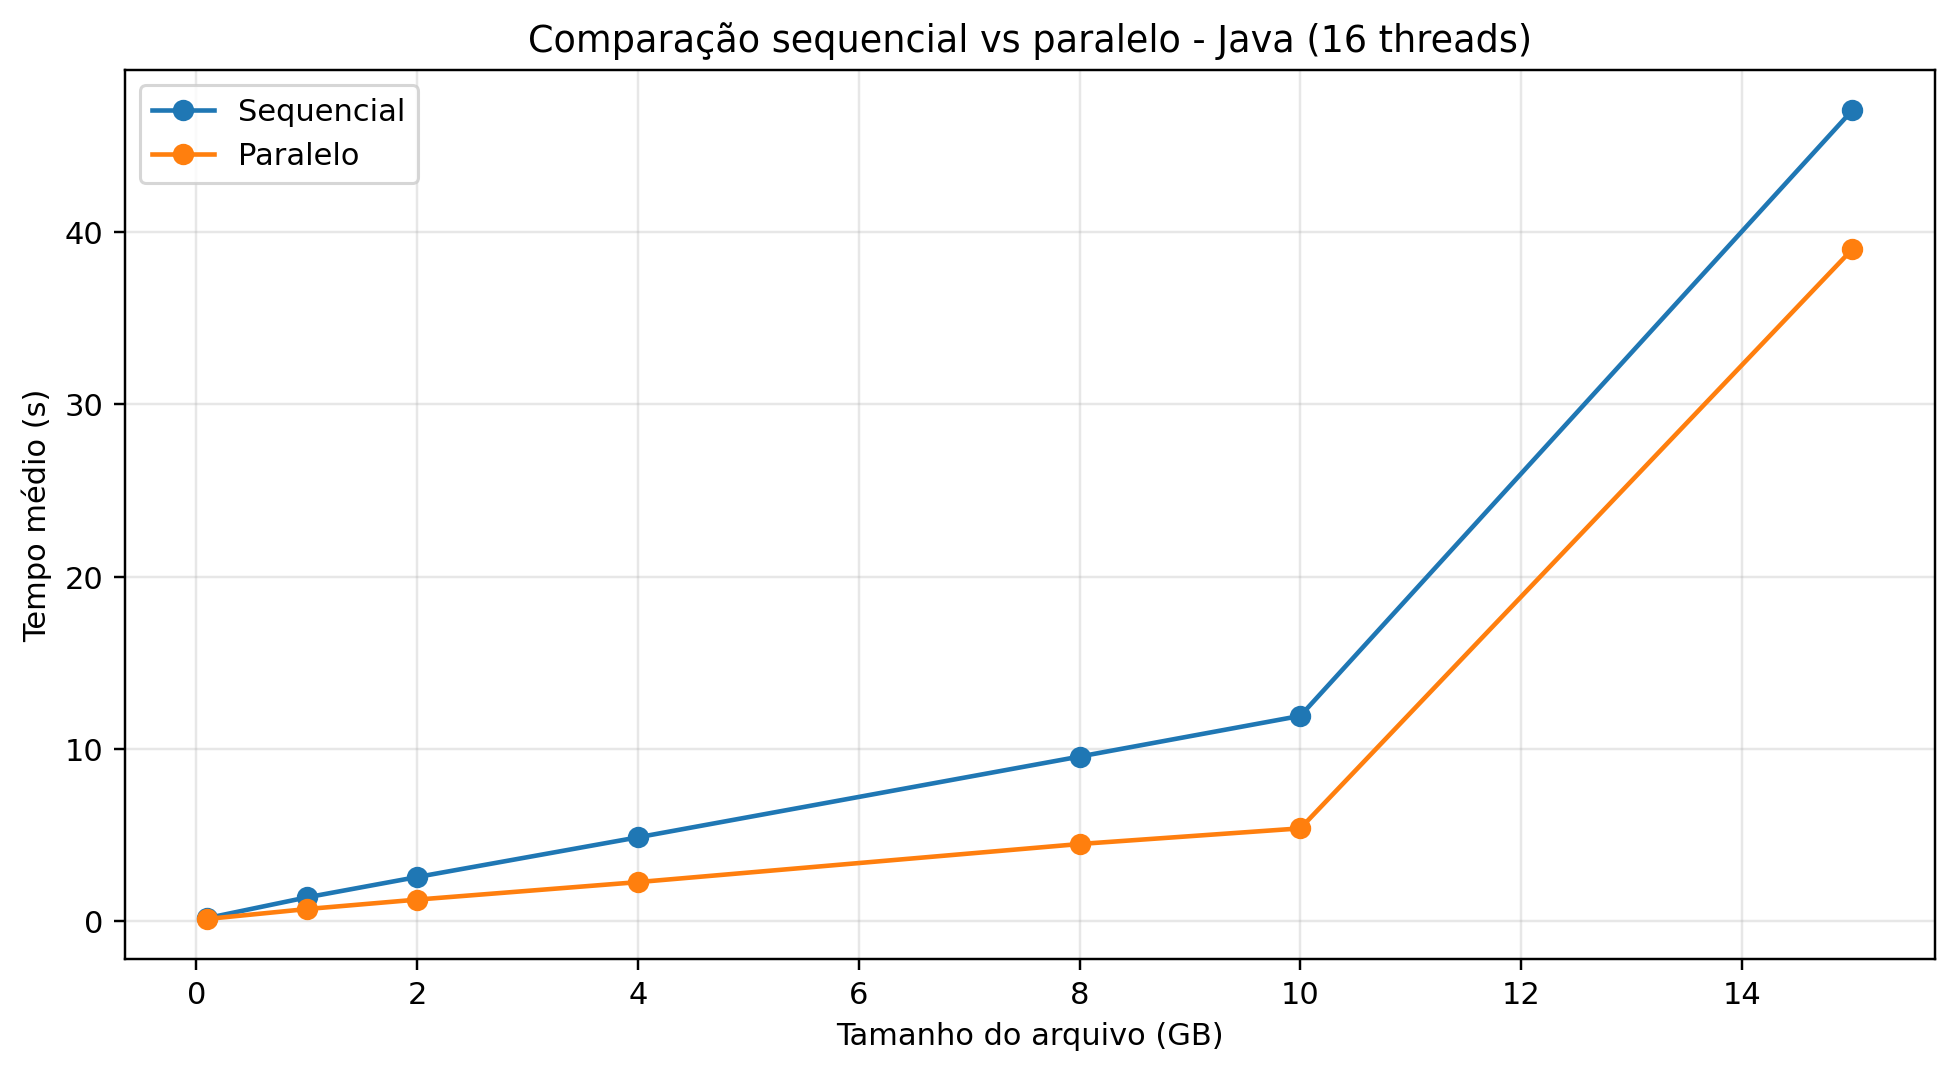
\includegraphics[width=0.45\textwidth]{graficos/comparacao_seq_vs_par_Java_16_threads.png}
\caption{Comparação entre execução sequencial e paralela em Java}
\end{figure}

% ------------------------------------------------
\section{Discussão}

A análise dos resultados obtidos evidencia diferenças claras entre as implementações em C e Java, bem como o impacto da paralelização no desempenho do problema.

Inicialmente, observa-se que a implementação em C apresentou desempenho superior em todos os cenários testados. Para arquivos menores, como 0,1 GB, a diferença já é perceptível, com o C executando aproximadamente duas vezes mais rápido que o Java. Essa diferença se mantém consistente conforme o tamanho do arquivo aumenta, sendo atribuída principalmente ao menor overhead da linguagem C e ao controle mais direto sobre memória e operações de baixo nível.

Em relação à paralelização, ambas as linguagens apresentaram ganhos significativos para arquivos de tamanho intermediário. O speedup observado variou entre aproximadamente 1,8x e 2,1x na maioria dos casos, indicando bom aproveitamento do paralelismo disponível. A implementação em C com OpenMP apresentou resultados ligeiramente superiores, especialmente para arquivos entre 2 GB e 10 GB, onde atingiu speedups acima de 2,1x.

Entretanto, para o maior arquivo testado (15 GB), houve uma queda significativa no ganho de paralelismo em ambas as linguagens, com speedup próximo de 1,1x. Esse comportamento indica a presença de gargalos relacionados à largura de banda de memória e ao custo de acesso ao armazenamento, limitando a eficiência do paralelismo. Nesse cenário, o aumento do número de threads não resulta em ganho proporcional de desempenho.

Outro ponto relevante é que o crescimento do tempo de execução não é perfeitamente linear com o tamanho do arquivo, especialmente nas versões paralelas. Isso ocorre devido a fatores como cache, comportamento do sistema operacional e gerenciamento de threads.

De forma geral, os resultados mostram que:

\begin{itemize}
    \item a linguagem C apresentou melhor desempenho em todos os cenários;
    \item o OpenMP proporcionou paralelização mais eficiente que threads em Java;
    \item o ganho de paralelismo é limitado por hardware em grandes volumes de dados;
    \item o algoritmo BMH mostrou-se eficiente e adequado para o problema.
\end{itemize}

\textbf{Inserir nesta seção a análise concreta dos gráficos e tabelas, destacando:}

\begin{itemize}[leftmargin=*]
    \item em quais cenários o C superou o Java;
    \item em quais cenários o paralelismo foi mais vantajoso;
    \item em que ponto o aumento do número de threads deixou de trazer benefícios;
    \item como o tamanho da palavra influenciou o desempenho;
    \item como a estratégia baseada em BMH se comportou em padrões curtos e longos.
\end{itemize}

% ------------------------------------------------

\section{Dificuldades Encontradas}

Durante o desenvolvimento das implementações, diversas dificuldades técnicas e conceituais foram observadas.

Uma das principais dificuldades foi garantir a corretude da contagem nas regiões de fronteira entre blocos e entre partições paralelas. Como a busca é por substring e não por palavra inteira, uma ocorrência pode iniciar em um bloco e terminar em outro, o que exige tratamento explícito de sobreposição.

Outro desafio importante foi evitar dupla contagem de ocorrências quando múltiplas threads inspecionam regiões adjacentes. A solução adotada nas implementações autorais foi o conceito de intervalo de propriedade, no qual cada thread é responsável apenas pelas ocorrências cujo índice inicial pertence ao intervalo que lhe foi atribuído.

Também houve dificuldades relacionadas à automação dos testes, incluindo:

\begin{itemize}[leftmargin=*]
    \item padronização da saída entre C e Java;
    \item correção de diferenças de locale na impressão de números em Java;
    \item integração com scripts Python para repetição de experimentos;
    \item interpretação correta dos dados exportados para CSV.
\end{itemize}

No caso da paralelização em Java, foi necessário ainda lidar com o custo de gerenciamento de threads e com a estrutura de \texttt{ExecutorService}. Já no caso do OpenMP, foi necessário ajustar a estratégia de divisão do trabalho e observar o impacto do número de threads sobre o desempenho final.

% ------------------------------------------------
\section{Conclusão}

Este trabalho apresentou a implementação e análise de soluções sequenciais e paralelas para o problema de busca de substrings em arquivos de grande porte, utilizando o algoritmo Boyer-Moore-Horspool como base comum.

Os resultados demonstraram que a implementação em C apresentou melhor desempenho geral, tanto na versão sequencial quanto na paralela. Isso se deve principalmente ao menor overhead da linguagem e ao maior controle sobre memória e operações de baixo nível.

A paralelização mostrou-se eficaz, especialmente para arquivos de tamanho intermediário, onde foram observados speedups superiores a 2x. No entanto, para arquivos muito grandes, o ganho de desempenho foi limitado por fatores de hardware, como largura de banda de memória e custo de acesso a disco.

A comparação entre Java e C evidenciou que, embora o Java ofereça maior abstração e portabilidade, o C ainda é mais eficiente para aplicações de processamento intensivo de dados.

Conclui-se que a melhor solução para o problema estudado foi a implementação paralela em C com OpenMP, por apresentar melhor desempenho e maior escalabilidade.

Como trabalhos futuros, destacam-se:

\begin{itemize}
    \item uso de técnicas SIMD e vetorização;
    \item comparação com outros algoritmos de busca;
    \item otimizações de cache e afinidade de threads;
    \item avaliação em diferentes arquiteturas de hardware.
\end{itemize}
% ------------------------------------------------

\begin{thebibliography}{99}

\bibitem{tanenbaum}
TANENBAUM, A. S.
\textit{Distributed Systems}. Pearson.

\bibitem{openmp}
OpenMP Architecture Review Board.
\textit{OpenMP Application Programming Interface}.

\bibitem{horspool}
HORSPOOL, R. N.
Practical fast searching in strings.
\textit{Software: Practice and Experience}, v. 10, n. 6, p. 501--506, 1980.

\bibitem{knuth}
KNUTH, D. E.; MORRIS, J. H.; PRATT, V. R.
Fast pattern matching in strings.
\textit{SIAM Journal on Computing}, v. 6, n. 2, p. 323--350, 1977.

\bibitem{java}
ORACLE.
\textit{Java Platform Documentation}.

\bibitem{gcc}
GNU Project.
\textit{Using the GNU Compiler Collection (GCC)}.

\end{thebibliography}

\end{document}